\documentclass[a4paper,11pt]{article}

\usepackage[ansinew]{inputenc}
\usepackage[french]{babel}
\usepackage[T1]{fontenc}
\usepackage[paper=a4paper, top=1cm, bottom=1cm, left=2cm, right=2cm]{geometry}
\usepackage{graphicx}
\usepackage{hyperref}
\usepackage{url}
\usepackage{xcolor}

\title{\large{\bfseries{ARCHITECTURE LOGICIELLE}}}
\author{Beno\^it V\'edrenne, Ga\"{e}l Walter}

\begin{document}

\maketitle

\begin{center}
\emph{Charg\'e de TD :} Damien Cassou\end{center}

\vspace{0.5cm}

\begin{center}

\includegraphics[width=2.5cm,height=2.5cm]{images/bdx1.eps}\\
\large{Universit\'e Bordeaux 1,\\
351 cours de la Lib\'eration,\\
33405 Talence Cedex,\\
France}
\end{center} 

\vspace{0cm}

\begin{center}
 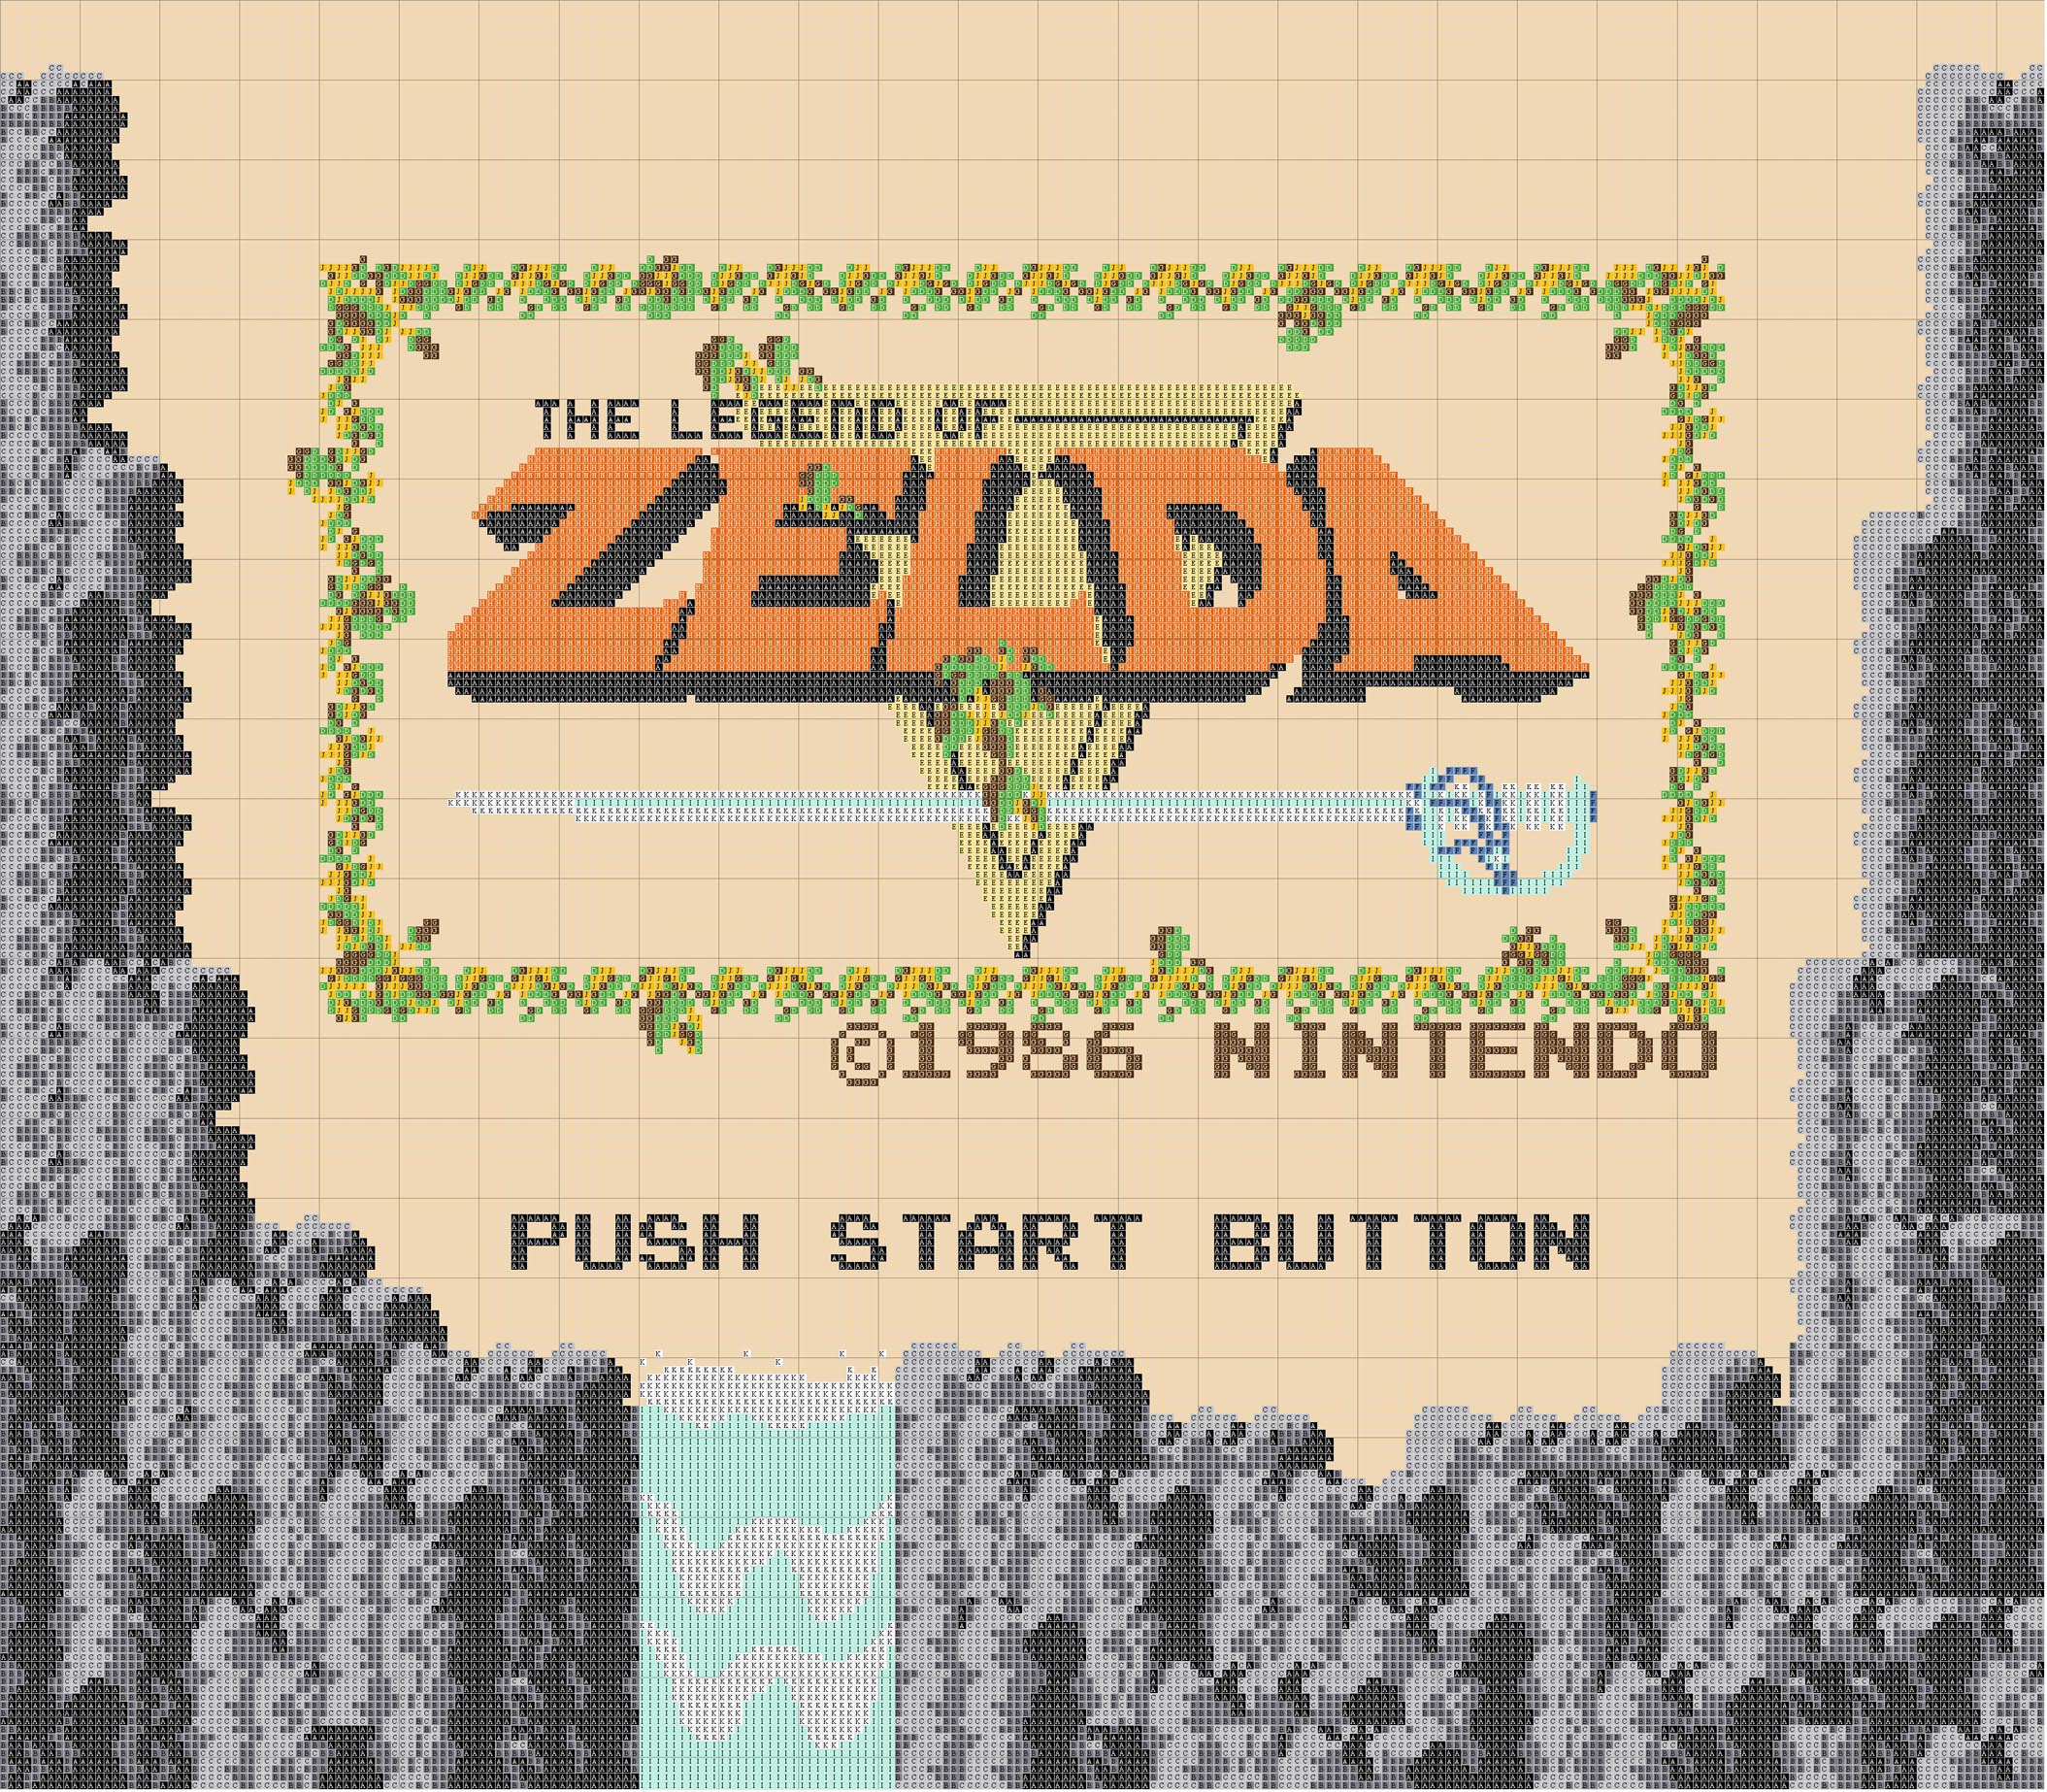
\includegraphics[width=9cm,height=9cm]{images/zeldaNintendo.eps}
\end{center}

\begin{center}
 \large{The Cremi Legend Of Zelda}
\end{center}

\begin{abstract}
La l\'egende raconte que la grande for\^et d'Hyrule est occup\'ee par Ganon, le
puissant Prince des T\'en\`ebres. Ganon a captur\'e la fille du Roi qui tenta de s\'eparer la
Triforce, puissant sortil\`ege qui prot\`ege le royaume d'Hyrule. Ses guardes
mal\'efiques avancent \`a grand pas dans la for\^et en d\'etruisant tout sur leurs
passages\ldots \\
Il existe cependant un chevalier courageux, en ces temps de manants. 
On le reconnait facilement \`a sa chevelure blonde sous sa longue cape
verte. Apprenant la nouvelle de l'invasion, le regard noir,
il parti dans les haut bois de la for\^et d'Hyrule pour les affronter tous et
lib\'erer la fille du Roi nomm\'ee ``Zelda''.\\

The ``CREMI Legend of Zelda'', c'est l'histoire de ce jeune garon, nomm\'e Link qui doit sauver la princesse Zelda au p\'eril de sa vie. \\
Une somme d'emb\^{u}ches l'attend. L'art de manier son \'ep\'ee pourra peut
\^etre l'aider dans sa qu\^ete impossible: seul contre une arm\'ee enti\`ere.
\end{abstract}

\newpage

\section{Introduction}

Le framework de jeu plateforme dont nous disposions, nous a permis
d'impl\'ementer une version du Jeu Zelda. Ce jeu, cr\'e\'e par Miyamoto (auteur
\'egalement de Donkey Kong et Mario), poss\`ede une version Nintendo de 1986. \\

Notre application s'inspire de cette version, o\`u l'on peut guider dans une
for\^et le personnage Link. \\
Nous l'avons bien s\^{u}r d\'enomm\'e Cremi Legend Of Zelda car il a \'et\'e
principalement d\'evelopp\'e au Cremi !

\subsection{Comment jouer \`a CLOZ ?}

Le but du jeu est de guider Link dans la for\^et pour l'amener \`a la
princesse Zelda avec les
touches fl\'ech\'ees. \\ 
On devra tout d'abord \'eliminer tout ses ennemis mal\'efiques en utilisant le coup
d'attaque par la touche ``Espace''. Ceux ci sont tr\`es \'enerv\'es car
ils ont \'et\'e pr\'evenus de l'arriv\'e de Link, c'est pour cela qu'ils n'ont pas un
comportement tr\`es logiques. Parfois, il se peut qu'un ennemi plus robuste
surveille plus raisonnablement Zelda, il est donc plus difficile \`a
tuer. Il ne faut pas h\'esiter \`a les frapper de mani\`ere r\'ep\'et\'ee.\\

La difficult\'e du jeu r\'eside dans le nombre d'ennemis \`a tuer, plus ou moins
forts selon leurs grades, mais aussi dans les diff\'erents objets
qui peuvent agr\'ementer le jeu. Le joueur est libre de tous les
essayer. Mais comme dans la r\'ealit\'e, les bombes blessent.\\

La vie de Link d\'emarre \`a ``100'' mais elle peut descendre tr\`es
vite ! Faites attention Link, n'est pas immortel. En mourrant, vous
recommencerez le jeu au d\'ebut du niveau.

\subsection{Quelques r\`egles du jeu}

Seul le clavier est utile au jeu, mais le menu permet d'autres actions.\\
Au croisement avec des ennemis, Link perd de la vie car il se fait
frapper par ceux-ci. Les boss notament sont plus coriaces (de vrais brutes), et
tapent plus fort. Si notre h\'eros meurt, le niveau de
jeu red\'emarre au d\'ebut. \\
Depuis le menu, on peut red\'emarrer la partie au d\'ebut, mais aussi sauvegarder la
partie ou (en th\'eorie) en restaurer une.\\
Lorsque tout les ennemis sont tu\'es, il faut aller vers la princesse et le
niveau est gagn\'e, on passe alors automatiquement au niveau suivant, s'il existe.
On peut trouver une arme sur le sol, Link peut attaquer avec. Il est possible
que certaines actions enl\`event cette arme, et le combat de boss devient plus
ardu.

\subsection{Astuces}
Comme dans beaucoup de jeu vid\'eo d'aventure, nous avons laiss\'e des codes
secrets que l'on peut chercher si l'on veut. Qu'il est agr\'eable en \'etant joueur
de trouver ce genre de code ! Mais n'oubliez pas que l'abus de codes nuit
au plaisir de jouer.

\newpage

\section{Conception}

La premi\`ere phase du projet ft d'\'etudier le framework donn\'e, ainsi que le code
du jeu Pacman. Le framework nous permet de cr\'eer un jeu bas\'e sur un univers
donn\'e, des entit\'es \'evoluant dans ce monde selon des r\`egles de collisions
donn\'ees. Nous avons commenc\'e  utiliser les classes du jeu Pacman pour d\'ebuter
Zelda. Ce f\^ut non seulement un moyen de comprendre plus vite comment utiliser
certaines fonctionnalit\'es du framework, mais aussi une difficult\'e de commencer
 vouloir adapter un jeu d\'ej\`a fait \`a un autre, plut\^ot que de partir sur une
base saine.\\
Ce choix nous amena \`a ajouter petit \`a petit les diff\'erentes fonctionnalit\'es en
plus que nous voulions.

\subsection{Pacquetages}

Au fur et  mesure de l'impl\'ementation, nous avons mis en place une
arborescence de paquetages de classes, s\'eparant bien chaque partie du code, ce
qui nous a permis de nous retrouver plus facilement tout au long du projet. On
retrouve ``\textbf{base}'', ``\textbf{game}'' comme dans le framework, mais
aussi ``\textbf{rule}', ``\textbf{entity}'' comme dans la version de Pacman.\\

Le paquetage ``\textbf{zelda}'' comprend plusieurs paquetages.\\
Le paquetage ``\textbf{base}'' permet de g\'erer l'int\'eraction utilisateur,
sons, gestion de mouvements de personnages.\\ 
Le paquetage ``\textbf{rule}'' contient les r\`egles de gestion de collisions ou blocages entre entit\'es du jeu.\\ 
Le paquetage
``\textbf{level}'' permet de g\'erer la mise en place des niveaux du jeu, de la
lecture de fichier pour les niveaux, \`a la cr\'eation de niveaux.\\ 
Le paquetage
``\textbf{game}'' contient les classes n\'ecessaires \`a la cr\'eation du jeu
(gestion de l'univers, sauvegarde de niveaux\ldots).\\ 
Le paquetage
``\textbf{observer}'' permet de g\'erer tout les observateurs du jeu.\\ 
Le paquetage ``\textbf{entity}'' poss\`ede toutes les classes de toutes les entit\'es 
pr\'esentes dans le jeu : personnages et d\'ecors. Dans les personnages, un paquetage 
est r\'eserv\'e aux \'etats de Link.\\

%\subsection{Architecture g\'en\'erale}


\begin{center}
 %\includegraphics[width=9cm,height=9cm]{images/archiGenerale.eps}
\end{center}

\subsection{Architecture d\'etaill\'ee}

\subsubsection*{Une Fabrique Abstraite pour cr\'eer le niveau depuis un fichier
texte}

Nous avons choisi d'utilis\'e une fabrique abstraite pour permettre la
cr\'eation et l'ajout d'entit\'es dans le niveau. Il \'etait assez intressant
de cr\'eer cette fabrique abstraite car ainsi nous ne faisions juste qu'une
demande de cr\'eation d'un certain objet qu'elle s'occupait d'instancier. Une
personne voulant cr\'eer un personnage ou une autre entit\'e a juste besoin de faire appel \`a la m\'ethode create ad\'equate. 
Cependant, le probl\`eme le plus important et qui est un probl\`eme propre \`a
ce mod\`ele est que l'ajout de nouvelles entit\'es est assez fastidieux : 
chaque nouvel objet il faut une m\'ethode pour le cr\'eer. Dans les constructeurs
de niveaux actuels il faut ajouter dans la table de hashage la m\'ethode associ\'ee.

\begin{center}
 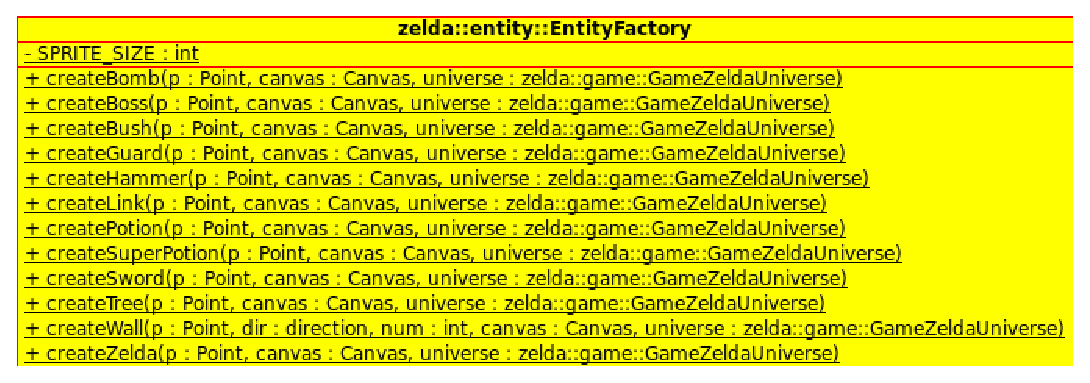
\includegraphics[scale=0.8]{images/Factorydiagram.eps}
\end{center}

On reconna\^it bien l\`a la structure d'une fabrique abstraite avec ses
diverses m\'{e}thodes de cr\'eation d'objet.

\subsubsection*{Le pattern Monteur pour sauvegarder la partie}

Le fait de sauvegarder la partie est une action classique de tout
jeu. Il nous est apparu comme \'evident d'avoir une repr\'esentation sur
fichier du contenu de cette sauvegarde. Nous avons donc mis en place un
monteur, celui-ci en effet est particuli\`erement adapt\'e \`a ce genre de
situation. Nous avons donc cr\'eer un monteur concret qui permet d'\'ecrire
un fichier texte contenant les informations ainsi sauvegarde.\\
Un autre avantage de ce patron de conception est que nous pouvons ainsi
rapidement modifier la repr\'esentation de cette sauvegarde. Il est tout \`a
fait possible d'imaginer une sauvegarde au format HTML ou XML, ou on ne
sait dans quel autre format. Le format de la sauvegarde est donc facilement
modifiable pour n'importe quelle personne reprennant notre code et qui
n'aimerait pas notre repr\'esentation. \\

\begin{center}
 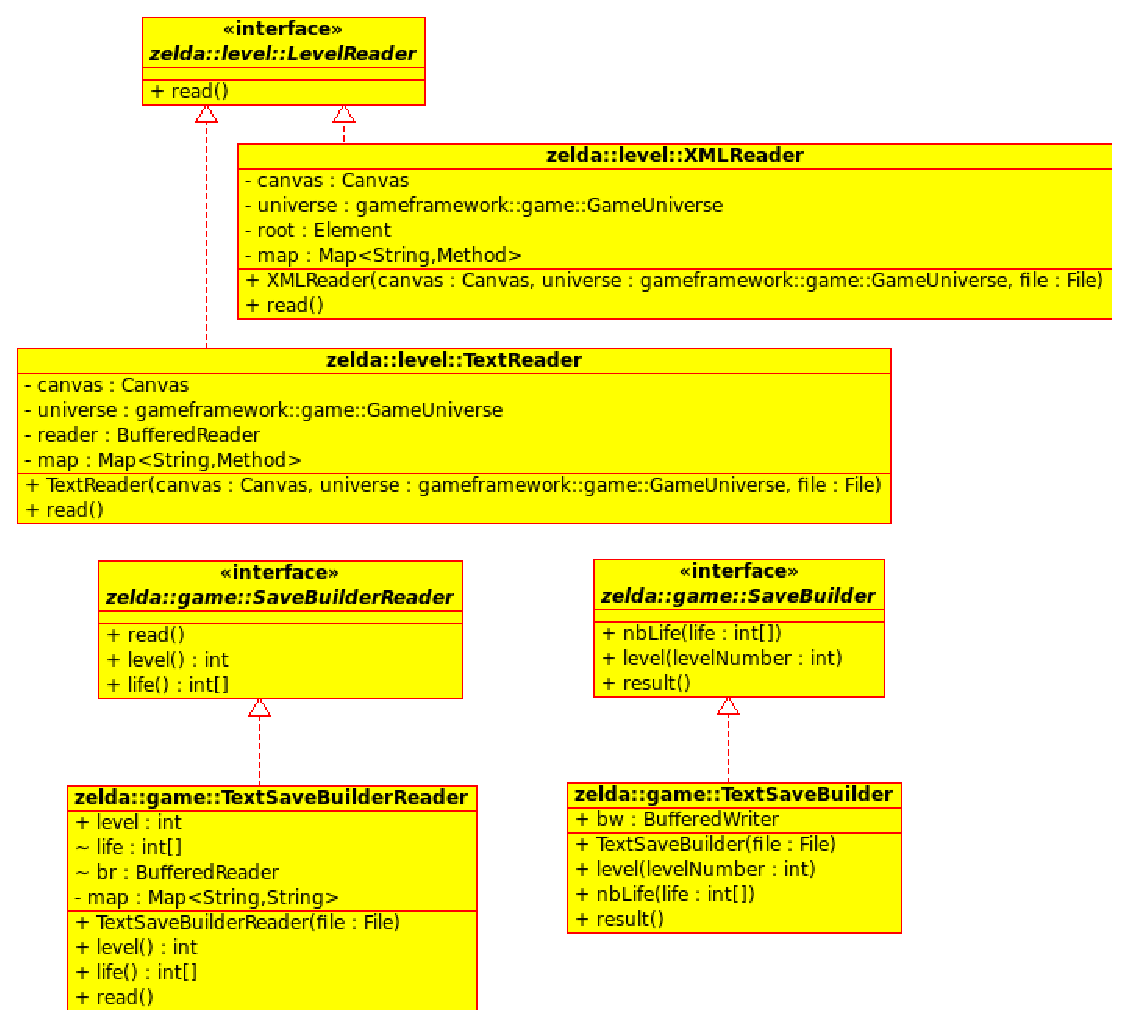
\includegraphics[scale=0.7]{images/Buildersdiagram.eps}
\end{center}

Nous avons aussi utilis\'e ce mod\`ele pour la lecture de la sauvegarde
ainsi que la lecture du fichier de cr\'eation de niveau et ce pour les
m\^{e}me raisons que celles \'enonc\'ees juste avant. Leur mise en place 
est visible sur l'image ci-dessus.\\
Sur cette image on voit bien les divers monteurs, on reconna\^it leur
m\'ethode de cr\'eation s\'equentielle. Il est donc facile de voir comment
\'etendre l'interface de chacun pour pouvoir changer la repr\'esentation
d'une partie de ce jeu.

\subsubsection*{Gestion des \'etats de Link avec le pattern Etat}

L'\'etat de Link modifie son comportement. Ces changements
apparaissent de faon dynamique, selon les \'evnements du jeu, ou du joueur.
Cette intention nous a amen\'e \`a utiliser le pattern Etat pour g\'erer Link. Celui
ci peut d\'el\'eguer son comportement changeant \`a une hi\'erarchie de classes
LinkState poss\'edant des requ\^etes sp\'ecifiques comme l'utilisation de l'arme, le
mode attaque, la mort du personnage\ldots
Sur la fin du d\'eveloppement, cette conception nous a permis de rajouter
rapidement de nouveaux \'etats, et d'ajuster le comportement voulu facilement. \\

\begin{center}
 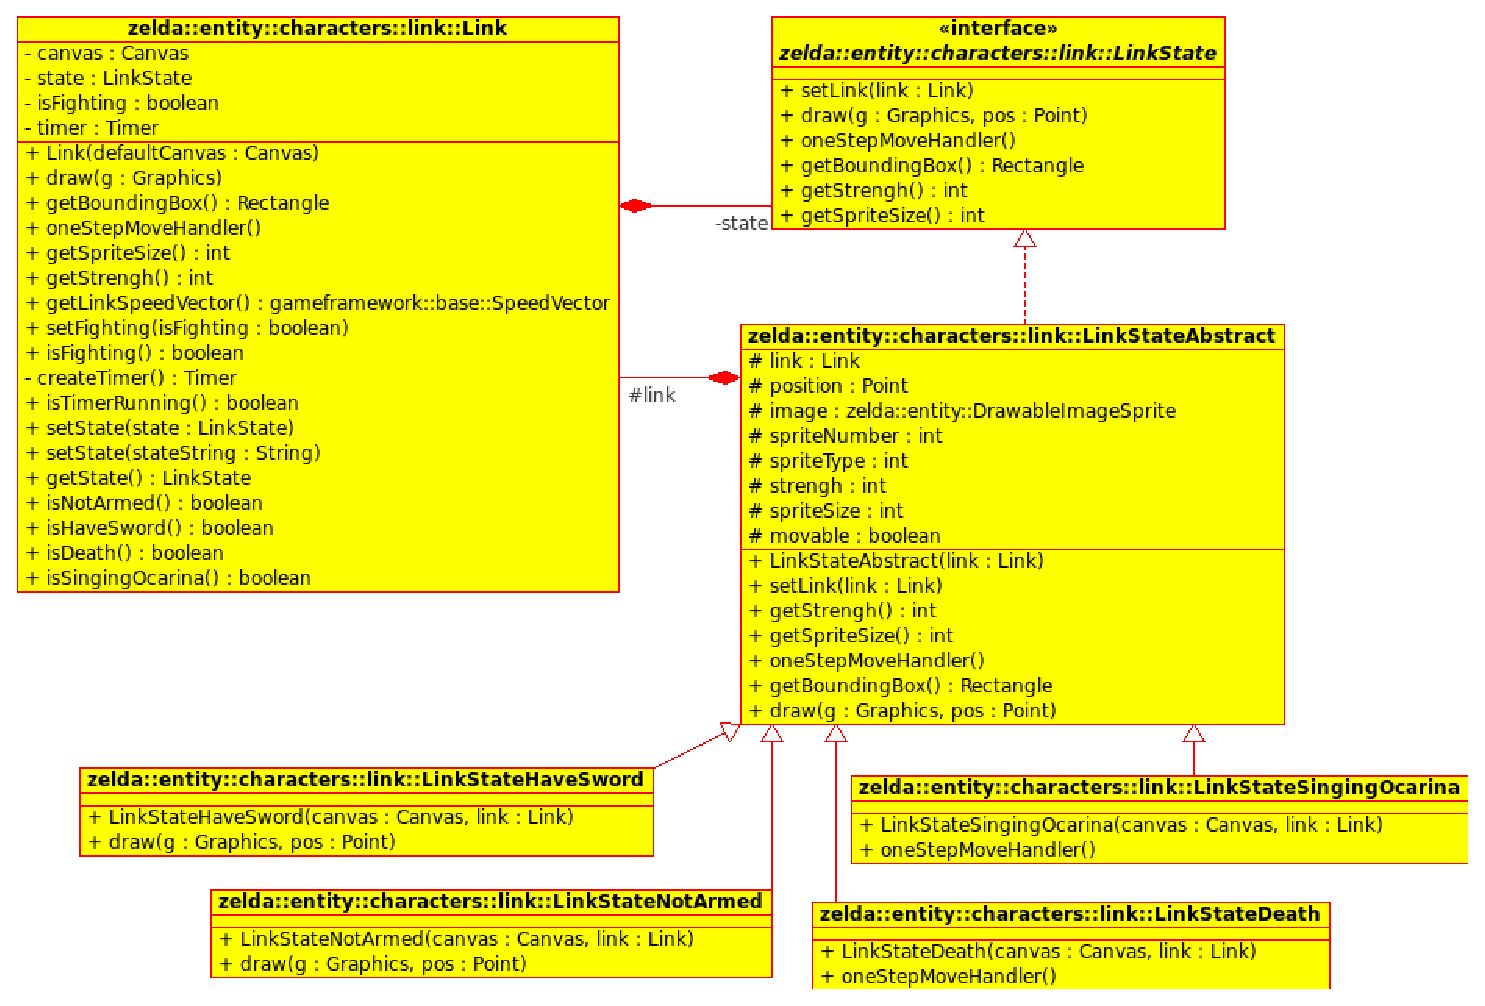
\includegraphics[scale=0.7]{images/Statediagram.eps}
\end{center}
 
\subsubsection*{un Singleton pour g\'erer le nombre d'ennemis dans le niveau}
Dans le jeu, une des priorit\'e est d'\'eliminer tous les ennemis afin de pouvoir
finir le niveau. Afin de g\'erer le nombre d'ennemis, on cr\'ee un observateur
unique  qui on adresse en d\'ebut de niveau le nombre d'ennemis \`a tuer.
L'int\'er\^et est ici de cr\'eer une unique instance d'observateur et de fournir un
point d'acc\`es global \`a celle ci depuis toutes les classes du jeu. L'utilisation
du mod\`ele Singleton f\^ut alors \'evident.

\begin{center}
 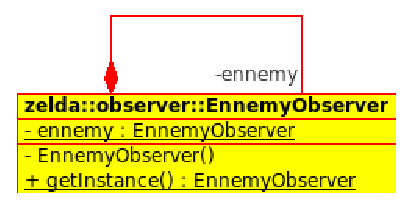
\includegraphics[scale=0.8]{images/Observerdiagram.eps}
\end{center}
 
\section{Evolutions}
Notre jeu Zelda n'est pas compltement fini, il ne comprend que quelques
niveaux, comprenant quelques ennemis, et quelques objets classiques. 
Quelques sprites ne sont pas parfaits, ni complets.\\
Cependant, le jeu fonctionne correctement, les fonctionnalits que nous
voulions au dpart tant implmentes.\\

Nous aurions voulu, avec plus de temps, produire des niveaux plus riches en
entit\'es, plus agr\'eables  jouer. Le jeu semble trop court, et nous aurions voulu
d\'evelopper un sc\'enario plus attractif.

\subsection{Critiques}
Le mouvement des gardes a \'et\'e honteusement copi\'e de celui des ``ghosts'' du Jeu
Pacman donn\'e, dans un premier temps, ce qui nous a permis de nous concentrer
sur d'autres \'el\'ements du jeu. Finalement nous nous sommes habitu\'es \`a ces
mouvements primitifs qui ajoutent une difficult\'e au jeu. Nous pourrions cr\'eer
une autre m\'ethode de d\'eplacement, plus intelligente, qui suivrait un
d\'eplacement pr\'ecalcul\'e. Une bonne aptitude des gardes serait de changer de
m\'ethode d\'eplacement et aller attaquer Link d\`es qu'il s'approche trop pr\`es de
Zelda ou trop pr\`es d'une zone donne.\\

Les sons ne sont pas assez nombreux, ce qui laisse une part de silence trop
grande, mais le systme de son est mis en place, ce qui nous relie aux besoins
du projet m\^eme.
 
\section{Impl\'ementation}

\subsection*{Probl\`emes rencontr\'es}

Nous avons bien sur rencontr\'e plusieurs points difficiles.

\subsubsection*{Gestion des niveaux}

Nous avons mis en place plusieurs niveaux ainsi qu'un changement de ceux-ci, 
ce qui s'av\'era \^etre une t\^ache ardu. En effet, nous pouvons passer au niveau 
suivant sans probl\`eme mais choisir au hasard un niveau et le lanc\'e est malheureusement
impossible. Nous avons voulu mettre en place un syst\^eme utilisant ceci via le rechargement
de sauvegarde. Avec notre impl\'ementation, quand nous rechargeons un niveau, le niveau se 
charge mais celui-ci ne d\'emarre pas. Nous avons tent\'e de diverse façon de faire en sorte que
cela fonctionne sans r\'esultat. En fait, le plus compliqu\'e vient de l'utilisation des threads
qui doivent \^etre interrompus avant de passer au niveau suivant et le niveau suivant doit \^etre
lanc\'e. Mais pour des raisons inconnus, les threads ne se lancent pas.

\subsubsection*{XML}

En th\'eorie, il est possible de cr\'eer des niveaux au format XML gr\^ace au Monteur LevelReader, malheureusement
nous avons eu des difficult\'es \`a mettre en place ce lecteur de XML. Nous n'avons pas r\'eussi surement 
\`a cause du fait que nous n'avions jamais utilis\'e l'API correspondante auparavant, et les diff\'erents 
tutoriaux pr\'esent sur internet n'ont pas suffit \`a nous permettre de r\'eussir.

\subsubsection*{Le framework de base}

Le fait d'\^etre confront\'e \`a un framework dont nous ne pouvions rien toucher, fut un challenge int\'eressant 
mais cependant parfois compliqu\'e. Il nous est arriv\'e \`a plusieurs reprise de vouloir r\'ecup\'erer une chose
d'une classe du framework, alors que cette chose ne nous \'etait pas accessible ou encore modifier une variable
priv\'ee inaccessible de l'ext\'erieur. Nous avons avoir parfois \'etait tent\'e par la recopie de code (ce que nous 
pouvons apercevoir avec la classe GameZeldaAWTImpl) mais il fallait le plus souvent trouv\'e des astuces. Ces astuces 
\'etaient souvent des mod\`eles de conceptions, par exemple nous avons utilis\'e un d\'ecorateur pour permettre d'\'etendre 
les fonctionnalit\'es d'une interface qui ne nous permettait pas de r\'ecup\'erer une variable pourtant essentielle 
sans laquelle le jeu aurait paru \'etrange aux yeux des divers joueurs.

\subsubsection*{Gestion des sprites}

Une des principales difficult\'es f\^ut de g\'erer correctement les sprites. Au
d\'epart, nous avions repris le code de Pacman. Celui ci utilisait pour Pacman
une grande image contenant une s\'erie de sprites diff\'erentes. Dans le code
apparaissait plusieurs fois le m\^eme identificateur SPRITE\_SIZE. Il nous a
fallu analyser plus en d\'etail le code pour nous rendre compte qu'en fait, tout
d\'ependait de la taille de l'image affich\'ee � l'\'ecran, de sa taille en largeur
et hauteur en pixels. Durant plusieurs jours, nous nous sommes ent\'et\'es �
utiliser des sprites complexes, de tailles vari\'ees. L'id\'ee f\^ut alors de cr\'eer
ses propres sprites et de s'occuper de chacun selon ses dimensions respectives.
\\ 
Ainsi pour Link, on a cr\'e\'e un sprite sans arme, et un autre avec \'ep\'ee. 
L'utilisation de plusieurs classes permet alors d'utiliser le sprite voulu avec
ses dimensions particuli\`eres, nottament le nombre de sprite sur une ligne,
mais aussi son affichage \`a l'\'ecran. \\
La difficult\'e f\^ut d'abord d'apprendre � utiliser le logiciel de retouches
d'images Gimp, ce qui ne f\^ut pas sans peine, sachant qu'il nou fallait peu de
temps pour cr\'eer une s\'erie de plusieurs sprites diff\'erents, cal\'es au pixel
pr�s. \\
Ensuite, il a fallut d\'em\'eler les SPRITE\_SIZE selon leur vraie utilit\'e. \\
Ensuite, il a fallu g\'erer l'utilisation du bon sprite selon l'\'etat du
personnage (pour Link). Link f\^ut le personnage qui f\^ut le plus compliqu\'e �
manier dans le sens o� justement les transitions d'\'etats compliquent la gestion
du mouvement des sprites selon la classe qui l'utilise. Il n'est pas impossible
par exemple que sur la derni\`ere version, les derni�res modifications aient
entrain\'ees que l'on ne puisse plus voir le sprite de Link en train de jouer un
air de musique, car on fait suivre ce mouvement particulier d'une nouvelle
transition d'\'etat vers un Link arm\'e par exemple. Surement que ce probl\`eme sera
d\'ebuggu\'e d'ici la remise du projet (en tout cas �a a march\'e il y a quelques
heures!).\\

Les sprites prirent donc un temps monstrueux dans la gestion du projet, ce qui
a affaibli les fonctionnalit\'es o� le design des autres entit\'es du d\'ecor. 

\end{document}
